\chapter{Introduction}
\par The presentation is the art of persuasion, It plays a significant role in our society and has the tremendous impact on the success of everyone \cite{seiler2002communication}. The presentation commonly used to communicate the presenter's ideas to the listener. However, giving a presentation successfully like John F. Kennedy or Steven Jobs is not a simple thing. A great preparation not only contains verbal style but also needs various nonverbal behaviors. On one hand, the content of a preparation must be clear, vivid and appropriate\cite{rodman1996style}. On the other hand, the significant component of a presentation lies upon nonverbal cues which have the power to change the meaning assigned to spoken words\cite{seiler2002communication}. 
\par Nonverbal behaviors of public speakers are expressed via several channels such as voice, gesture and facial expression. They have been proven to have a more significant influence than verbal cues. According to Argyle nonverbal messages are thirteen to fourteen times more powerful than verbal ones\cite{argyle1971communication}. Likewise, Arcy showed that the audience receives more than half of information from nonverbal behaviors\cite{d1998communicating}. The study of Seiler\cite{seiler2002communication}shows the fact that most people unconsciously believe more in nonverbal behaviors than verbal cues.
\par Unfortunately, it's hard to practice to express the effective nonverbal behaviors because they are mostly expressed subconsciously. To achieve the learning results, trainees must be provided with appropriate feedbacks from human advisors, but it is costly and not always available. According to Seiler \cite{seiler2002communication}, imitation is a kind of effective method to help the trainee to refine their nonverbal behaviors. Imitating those past famous speakers' gesture, sound or enunciation to learn what they're doing right, and then try to make it your own as Pablo Picasso said \emph{`` Good Artists Copy. Great Artists Steal "}. It is a great learning experience and can stretch trainees' abilities.
% because it requires certain skills\cite{rosenberg2005acoustic}. One aspect is the preparation of the presentation draft in advance, it can be relatively easily refined by revising the presentation draft many times by theirselves. Many books and tutorials have been written through training. The other is the way the orator delivers the presentation to others. It is difficult to be refined because they need to practice for many times and get some advice from the professionals to know their shortcomings, and it will cost a lot of time and money. 

\par In parallel, the role of nonverbal behaviors in computing is becoming increasingly recognized by the development of the emerging fields, such as social signal processing and affective computing. Such as \cite{Chen,cao2017realtime,Fang2016,Papandreou2017,He2017}, those Deep Learning library can extract user's body key point with high accuracy. Therefore, computers have been equipped with the abilities to decode the complexity of humans nonverbal channels. 

\par Many papers discussed some approaches toward the automatic recognition of nonverbal from trainees. However these approaches all defined some exact rules in advance to give a score of the presentation, but few have focused on imitating past famous speech to refine their nonverbal behaviors. 
 
\par In this paper, we propose a presentation training system that allows the trainee to imitate past famous speech to improve their nonverbal behaviors. Nonverbal behaviors include many aspects, and we choose to analyze the gesture of orators as the nonverbal behavior in this paper. In advance, we employed OpenPose library\cite{cao2017realtime} to extract orators' motion data from past famous speech 2D video. While training, the system capture the trainee's motion in real-time using Microsoft Kinect. We choose the cosine similarity of adjacent limbs as the feature to calculate the score that shows the similarity of the trainees' motion and the motion of extracted orators. The trainees will also wear an HMD that show a virtual hall and some virtual audience. The audience will perform some actions according to the score.
\begin{figure}[htbp]
\centering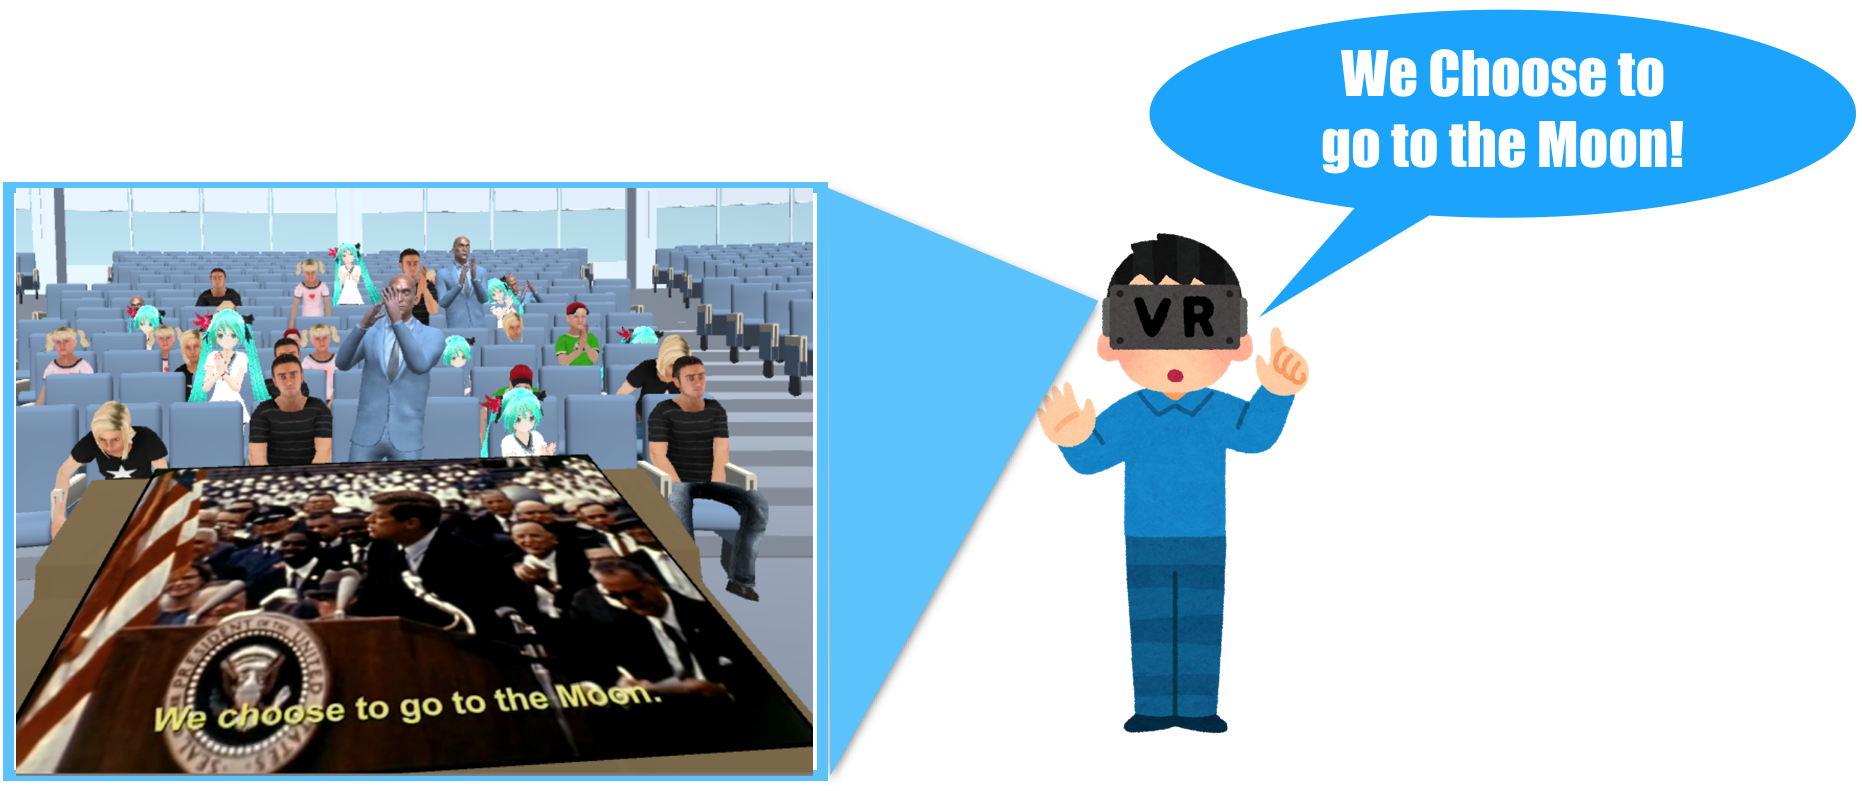
\includegraphics[scale=0.225]{./img/Introduction.png}
\caption{System Introduction}\label{fig:System Introduction}
\end{figure}

\par The rest of this paper is organized as follows. First we will introduce some existing presentation training method and proposed solution in the chapter 2. Then we will introduce the preparation about OpenPose, Kinect and the Evaluation of presentation in the chapter3. The chapter 4 describes our proposed system in detail. In the chapter 5, we will evaluate the system and discuss the results. The last chapter is for conclusions and future works.
